\section{Trabalhos Correlatos}
\label{subsection:trabalhoscorrelatos}
 Segundo \citeonline{tahawalid2009}, existem duas maneiras diferentes pelas quais um domínio pode ser definido. A primeira é quando o domínio está bem definido matematicamente, a segunda quando o domínio é definido por atividades puramente humanas. As DSLs de domínio humano, definem uma linguagem especial ou jargões para comunicar ideias relacionadas ao seu domínio.  
 
 Nesse contexto, os trabalhos correlatos encontrados mostraram formas de abstrair conceitos e jargões envolvendo questões legais, contratuais e regras sobre domínios financeiros. Os domínios dessas DSLs foram definidos com objetivo de apoiar na compreensão de atividades humanas e não de tratar de problemas computacionais ou matemáticos.
 
 Para tanto, as DSLs descritas nas próximas Seções foram encontradas por meio da busca pelas palavras-chave (domain specific languages, DSL, law e legal)  nos repositórios, \textit{Researchgate}, \textit{Google Scholar} e \textit{IEEEXplore}.
 
 
\subsection{LegalLanguage}
\label{legallanguage}

A DSL \texttt{LegalLanguage} é resultado da análise de ontologias que tratam de estrutura de documentos legais, sua construção busca estabelecer modelos conceituais com propósito de melhoria de comunicação e aprendizado sobre definições encontradas em textos normativos.

\begin{figure}[ht!]
\centering

\caption{\textmd{Modelo da DSL LegalLanguage}}
\label{fig:legallanguagemodel}
\fcolorbox{gray}{white}{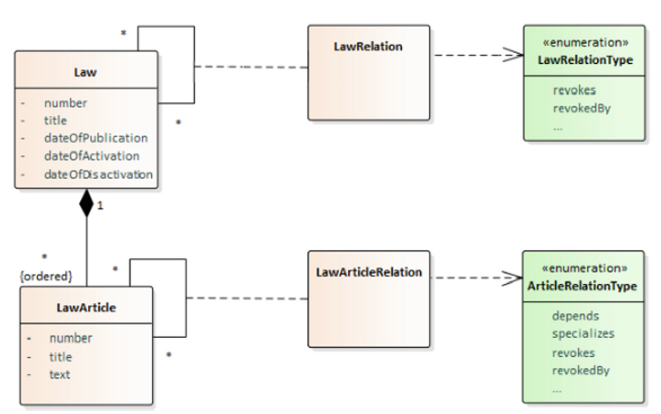
\includegraphics[width=0.90\textwidth]{chapters/trabalhoscorrelatos/imagens/legallanguagemodel.png}}

\par\medskip\textbf{Fonte:} \cite{legallanguage}. \par\medskip

\end{figure}



Segundo \citeonline{legallanguage}, o seu modelo é composto de \textit{Laws}, que podem ser classificadas como: Leis internacionais, regulamentos públicos, regulamentos privados, constituições e leis ordinárias. As leis são compostas por uma série artigos ordenados sequencialmente, os quais são organizados em divisões. É possível criar relacionamentos hierárquicos entre artigos de diferentes elementos de lei, bem como indicar revogações quando novas leis surgem (Figura \ref{fig:legallanguagemodel}). 

Segundo \citeonline[p.45, tradução nossa]{legallanguage}: "O desenvolvimento dessa linguagem tem como objetivo apoiar parlamentares que executam atividades inseridas em processos legislativos de redação de leis". Portanto, os autores à criaram utilizando a ferramenta \texttt{Xtext}, um exemplo de definição e uso do elemento \texttt{Law} pode ser observado nas Figuras \ref{fig:xtextlegal} e \ref{fig:legallanguageexample}.

\begin{figure}[ht!]
\centering

\caption{\textmd{Definição do elemento Law na LegalLanguage}}
\label{fig:xtextlegal}
\fcolorbox{gray}{white}{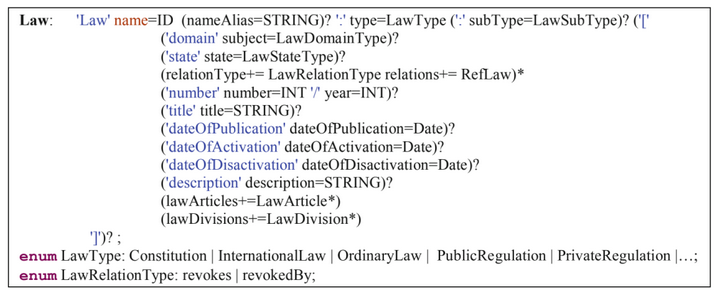
\includegraphics[width=\textwidth]{chapters/trabalhoscorrelatos/imagens/xtextlegal.png}}

\par\medskip\textbf{Fonte:} \citeonline{legallanguage}. \par\medskip

\end{figure}




\begin{figure}[ht!]
\centering

\caption{\textmd{Exemplo ilustrativo da LegalLanguage}}
\label{fig:legallanguageexample}
\fcolorbox{gray}{white}{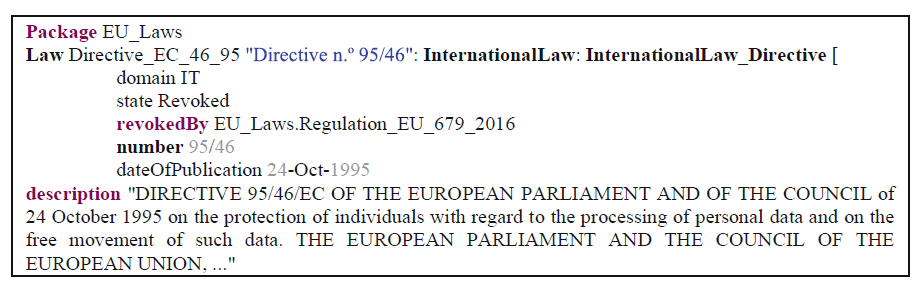
\includegraphics[width=\textwidth]{chapters/trabalhoscorrelatos/imagens/legallanguageexample.png}}

\par\medskip\textbf{Fonte:} \citeonline{legallanguage}. \par\medskip

\end{figure}





\newpage
\subsection{Ergo uma \textit{DSL} para Contratos Legais Inteligentes}
\label{ergo}

Ergo é uma linguagem específica de domínio que faz parte do projeto Accord, o qual define a base jurídica e técnica para contratos legais inteligentes, com objetivo de atender à problemas relacionados a falta de padronização em contratos legais. 

Segundo \citeonline{accordproject}, a linguagem tem o foco de ajudar desenvolvedores da área de tecnologia jurídica na escrita de contratos legais que possam ser computados. Um contrato legal inteligente é um contrato legível por seres humanos e por máquinas, por exemplo, uma clausula de cobrança de pagamento pode estar presente em um contrato, de modo que se possa utilizar o texto descrito em linguagem natural, para extração dos dados de cobrança e posterior aplicação de cálculos de multas e geração de eventos de notificações. 


É uma linguagem fortemente tipada e independente de plataforma, seu código pode ser compilado nas plataformas \texttt{JavaScrit} e \texttt{Java}. Ela prove uma linguagem de expressões, pela qual é possível descrever funções e clausulas de modo que possa ser definida a lógica de contratos inteligentes. 

Um exemplo de linguagem natural pode ser observado na Figura \ref{fig:ergotexto}, no qual os dados sobre a clausula de cobrança são mapeados, para posteriormente serem modelados e terem a lógica de cobrança seja definida (Figuras \ref{fig:ergomodelo} e \ref{fig:ergologica}). 

\begin{figure}[ht!]
\centering

\caption{\textmd{Exemplo ilustrativo da Ergo DSL}}
\label{fig:ergotexto}
\fcolorbox{gray}{white}{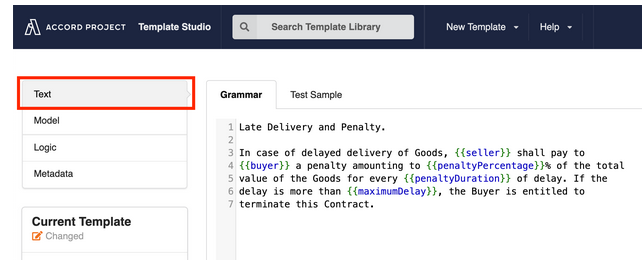
\includegraphics[width=\textwidth]{chapters/trabalhoscorrelatos/imagens/ergotexto.PNG}}

\par\medskip\textbf{Fonte:} \cite{accordproject}. \par\medskip

\end{figure}



\begin{figure}[ht!]
\centering

\caption{\textmd{Modelagem de clausula na ERGO DSL}}
\label{fig:ergomodelo}
\fcolorbox{gray}{white}{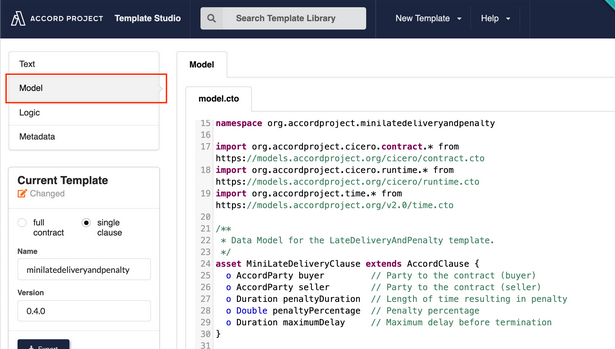
\includegraphics[width=0.90\textwidth]{chapters/trabalhoscorrelatos/imagens/ergomodelo.PNG}}

\par\medskip\textbf{Fonte:} \citeonline{accordproject}. \par\medskip

\end{figure}



\begin{figure}[ht!]
\centering

\caption{\textmd{Definição da lógica de contratos}}
\label{fig:ergologica}
\fcolorbox{gray}{white}{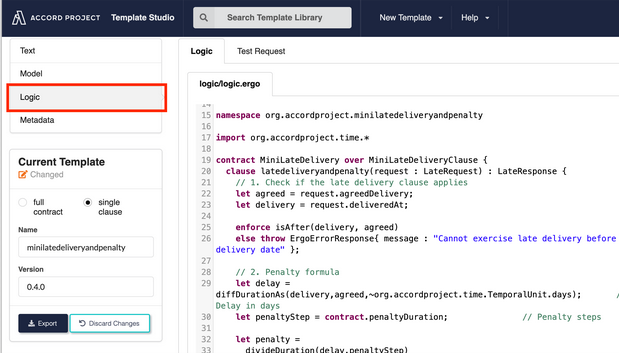
\includegraphics[width=\textwidth]{chapters/trabalhoscorrelatos/imagens/ergologica.PNG}}

\par\medskip\textbf{Fonte:} \citeonline{accordproject}. \par\medskip

\end{figure}



\newpage

\subsection{DSLFIN uma \textit{DSL} para sistemas financeiros}
\label{dslfin}